% !TEX encoding = UTF-8
% !TEX program = pdflatex
% !TEX root = InformationRetrieval.tex
% !TEX spellcheck = it-IT

% 14 Ottobre 2016

% section Ranking

\subsection{Strutture dati per la ricerca testuale}

La ricerca testuale ha delle caratteristiche che la rendono diversa dalla altre aree dell'informatica, non basta il \texttt{LIKE} delle query SQL, ma servono delle strutture dati specifiche.

Una di queste è l'indice trasposto o \textbf{inverted index}. Si tratta più di una famiglia di strutture dati, perché l'implementazione varia in base ad altri parametri, come la funzione di ranking che si vuole utilizzare. Tuttavia, tutte le possibili implementazioni hanno lo stesso scopo e lo stesso approccio al problema.

Il fatto di avere la struttura dell'inverted index correlata alla funzione di ranking permette di effettuare l'ordinamento dei risultati in modo efficiente.

\subsection{Query processing}

La gestione dei termini indice influenza l'elaborazione delle query degli utenti, è quindi importante effettuare un query processing efficiente visto che occorre gestire numeri consistenti di documenti.

La strategia di query processing dipende dal modello IR che viene adottato e che influenza la scelta della tipologia di indice trasposto da adottare. 
Si può sempre scegliere di utilizzare più indici trasposti in modo da supportare algoritmi diversi di query-processing.

Ovviamente non ha senso prendere in considerazione un modello IR che non permette di effettuare query processing in modo efficiente ed efficace.

\subsection{Un modello astratto}

Per introdurre le strutture dati degli indici trasporti ci baseremo su un modello astratto di ranking dei risultati.

\begin{figure}[htbp]
	\centering
	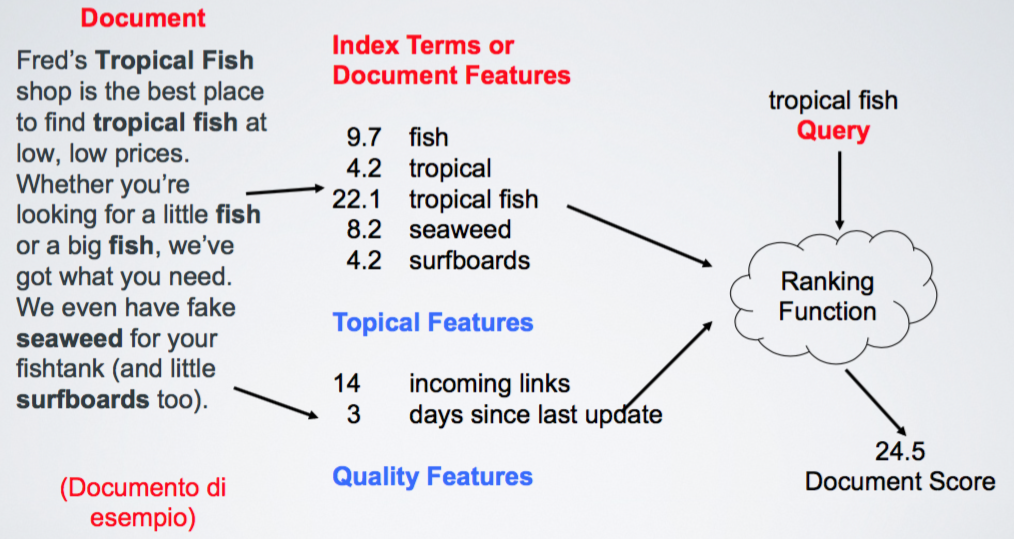
\includegraphics[width=0.6\textwidth]{./images/l6-modello}
\end{figure}


\noindent Abbiamo quindi un modello di indicizzazione che fornisce a determinate parole o frasi nei documenti un certo punteggio. Per il momento non ci preoccupiamo di come questi vengano calcolati.

Un altro sinonimo di termini indice è \textbf{features} che deriva più dall'apprendimento automatico.

Nel nostro modello di ranking d'esempio vengono prese in considerazione due categoria di features, quelle \textbf{topical}, che riguardano il contenuto (topic) del documento, e quelle \textbf{quality}, che descrivono delle qualità/caratteristiche del documento, come il numero di link entranti o i giorni dall'ultimo aggiornamento.

Una possibile funzione di ordinamento è data da:

$$
R(Q,D) = \sum_i g_i(Q) f_i(D)
$$

\noindent dove:
\begin{itemize}
	\item $f_i$ è una funzione che tiene presente le caratteristiche (\textbf{feature function}) del documento e che estrae un valore numerico per ogni caratteristica del documento.
	\item $g_i$ è una funzione simile ad $f_i$ che tiene presente le caratteristiche della query e che estrae un valore numerico per ogni caratteristica della interrogazione.
\end{itemize}

\noindent Come già detto, il calcolo della funzione di ranking viene fatto on-line.

Il risultato della sommatoria è quindi il punteggio del documento (\textbf{document score}) rispetto alla query e viene utilizzato per ordinare i documenti della collezione.

Da notare che nella sommatoria gli indici $i$ riguardano le caratteristiche della query, quindi se delle feature dei documenti non compaiono nella query, queste non vengono prese in considerazione.

\begin{figure}[htbp]
	\centering
	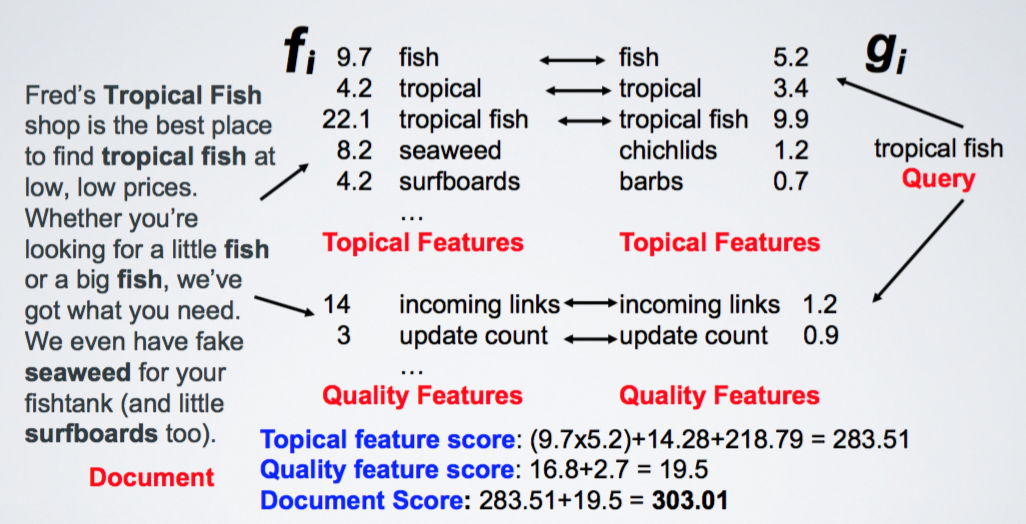
\includegraphics[width=0.6\textwidth]{./images/l6-modello-2}
	\caption{Le Topical features della query che sembrano ``extra'' sono aggiunti dal modello di indicizzazione che è una black-box. Tipicamente quelle extra vengono aggiunte dal modello perché riconosce che sono spesso utilizzate assieme alla query o perché derivano da possibili errori di battitura. Le quality features invece funzionano da \textbf{pesi} per le quality features dei documenti.}
\end{figure}

\subsubsection{Inverted Index e posting}

Ricapitolando: l'indice serve alla memorizzazione dell'elenco delle parole presenti nei documenti e viene prodotto dalla fase di indicizzazione, tuttavia i sistemi moderni utilizzano l'inverted index. 

\todo{a 1.04 potrebbe esserci qualcosa riguardo ai test}

Il ranking model considera che ogni documento è composto da feature e nell'inverted index ogni parola corrisponde ad una feature, segue quindi che l'inverted index viene utilizzato per calcolare lo score di un documento.

Ricapitolando: ogni termine indice (index term) ha la sia lista trasposta (inverted list) che mantiene i dati relativi al termine.
Ogni elemento di questa lista viene chiamato \textbf{posting} e contiene varie informazioni che possono essere utilizza per calcolare in modo efficiente lo score del documento, tra queste informazioni c'è un riferimento al documento di appartenenza che prende il nome di \textbf{pointer}.
Ogni pointer fa riferimento al documento mediante il suo identificativo univico, che non è detto sia un numero intero.

Quasi sempre le informazioni dei posti sono ordinate in base al numero dei documenti perché per certe funzioni i calcoli possono essere effettuati in modo più efficiente oppure la risulta più semplice comprimerle.

Un altro vantaggio dell'inverted index è quello che per rispondere ad una query non è necessario scorrerlo tutto, ma basta considerare il sotto-insieme relativo ai termini che compaiono nella query.

\subsubsection{Esempio di indice trasposto}
Documenti di partenza:
\begin{itemize}
	\item \textbf{S1}: Tropical fish include fish found in tropical environments around the world, including both freshwater and salt water species.
	\item \textbf{S2}: Fishkeepers often use the term tropical fish to refer only those requiring fresh water, with saltwater tropical fish referred to as marine fish.
	\item \textbf{S3} Tropical fish are popular aquarium fish, due to their often bright coloration.
	\item \textbf{S4} In freshwater fish, this coloration typically derives from iridescence, while salt water fish are generally pigmented.
\end{itemize}

\noindent L'indice trasposto più semplice è quello che contiene solamente gli identificativi dei documenti in cui compaiono i termini.

\begin{figure}[htbp]
	\centering
	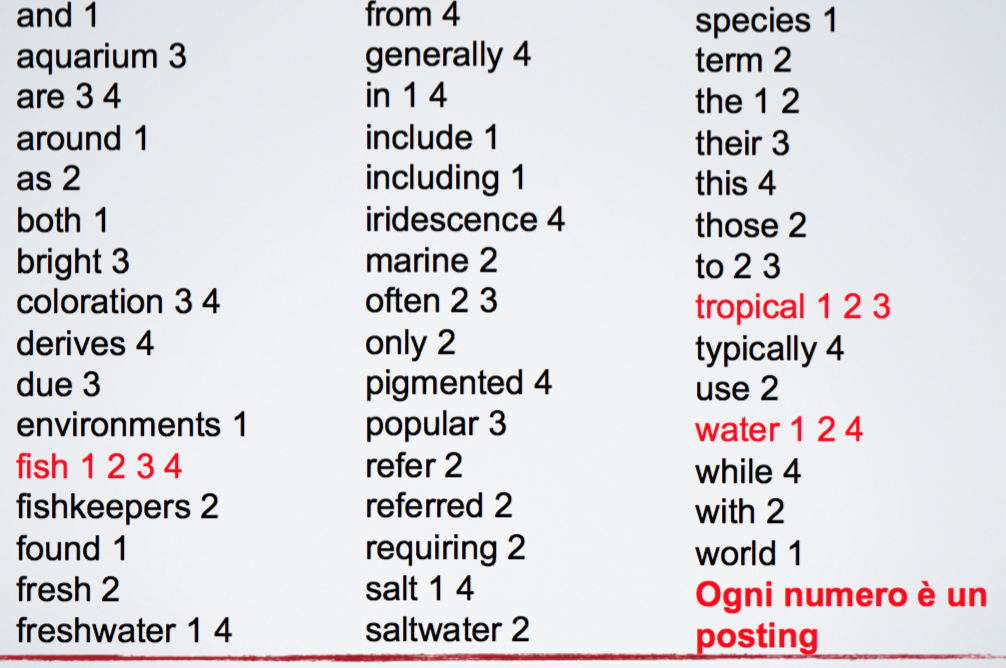
\includegraphics[width=0.6\textwidth]{./images/l6-index-1}
	\caption{Indice contenente solamente le informazioni riguardo a dove compaiono i termini.}
\end{figure}

\noindent Considerando la query \textit{``tropical fish''} e l'indice precedente verrebbero forniti come risposta i documenti \textbf{S1}, \textbf{S2} e \textbf{S3}, senza avere idea di quale possa essere il migliore.

Considerando anche la frequenza dei termini (\textbf{TF}) si ottiene un indice più complesso, come il seguente.

\begin{figure}[htbp]
	\centering
	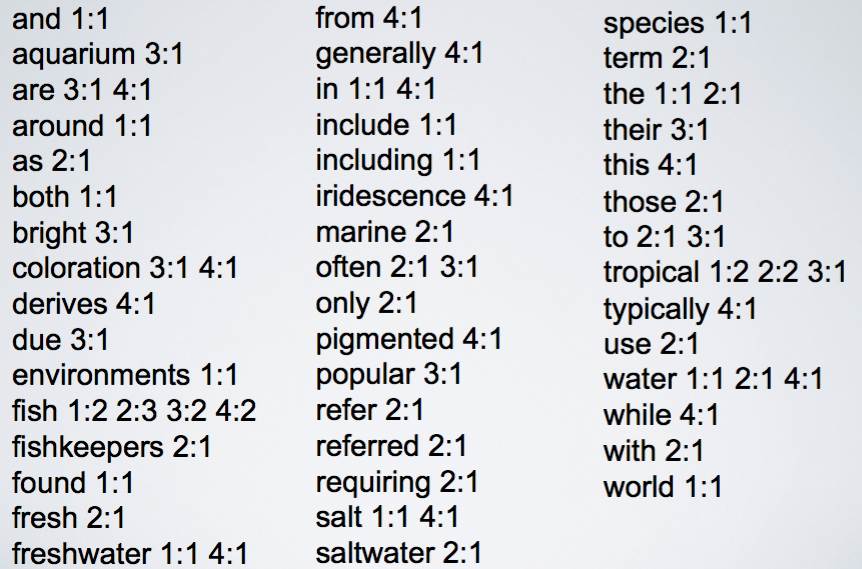
\includegraphics[width=0.6\textwidth]{./images/l6-index-2}
	\caption{Indice contente anche la frequenza dei termini.}
\end{figure}

\noindent Con le informazioni relative alla frequenza riusciamo a dare maggiore importanza al documento \textbf{S2} dato che contiene più volte i vari termini.

Anche se questo sistema è molto semplice si è comunque dimostrato efficace.



